\documentclass[12pt]{article}

\usepackage{graphicx}%import graphics


\begin{document}

\title{Bikeshare Data}

\author{Thayer Adsit, Matthew Chen, Cindy Huynh, James Leung}

\maketitle

\section{Introduction}
We look at general trends in the capital bikeshare system using both weather data provided by kaggle and bike usage microdata released by the capital bikeshare system. From the bikeshare microdata we can determine the general growth of the system. We also look at difference i usage patterns for registered and unregistered users of the system.

With the weather data we are able to determine the effects of different weather variables on bikeshare demand over a two year period.

Things to do would be to complete the list of question that we posed in the beginning of the exercise and possibly merge other datasets for further insight. An interesting comparison would be to compare this data to ones released by new york and their bike share system. Other questions posed during our coffee shop session are as follows:

\begin{enumerate}
	\item drunk biking around dc
	\item specific trips that people are making
	\item same route every day
	\item revenues of bikeshare
	\item average lifespan of a bike
	\item average speed of a rider over trip
\end{enumerate}


\section{General Trends}


\begin{minipage}{.5\textwidth}
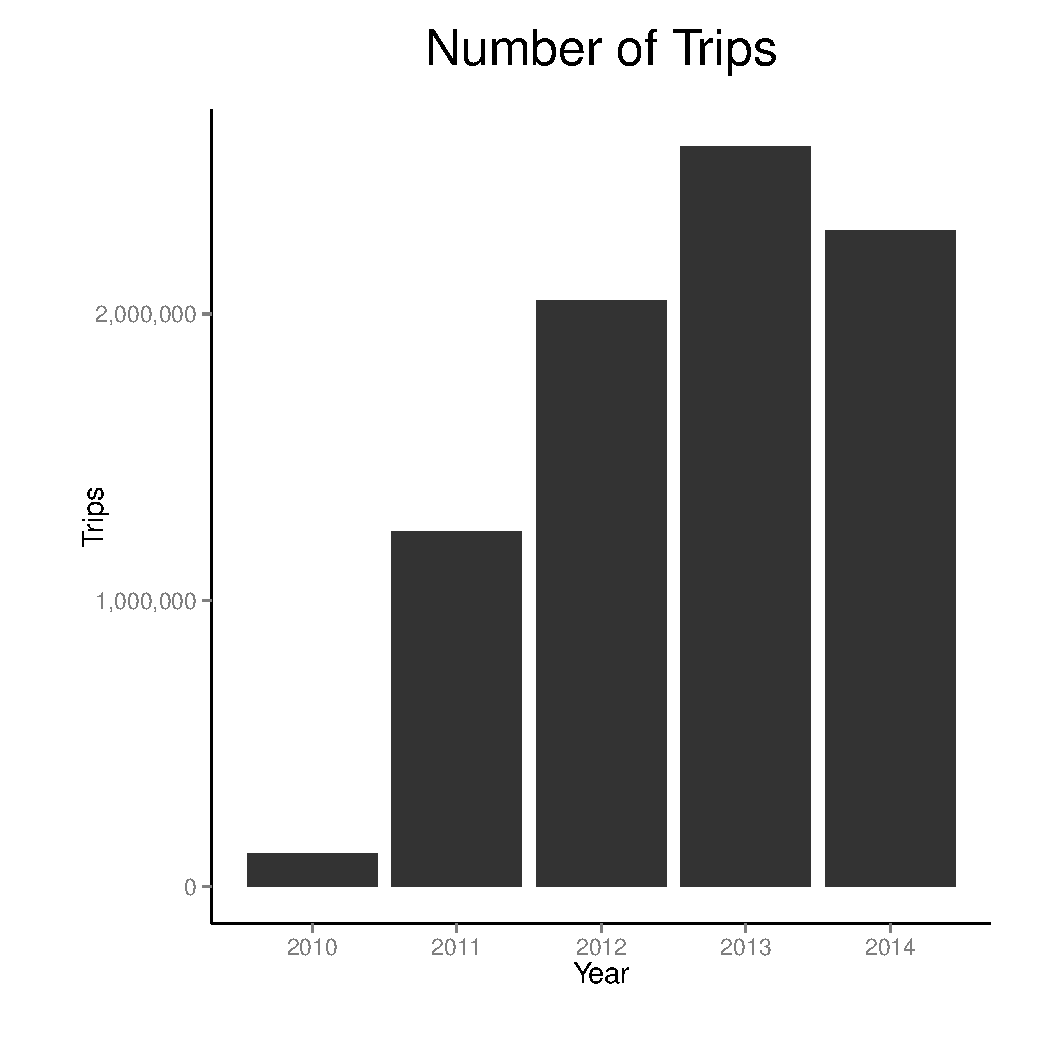
\includegraphics[scale=0.5]{../graphs/num_trips.pdf}
\end{minipage}%
\begin{minipage}{.5\textwidth}
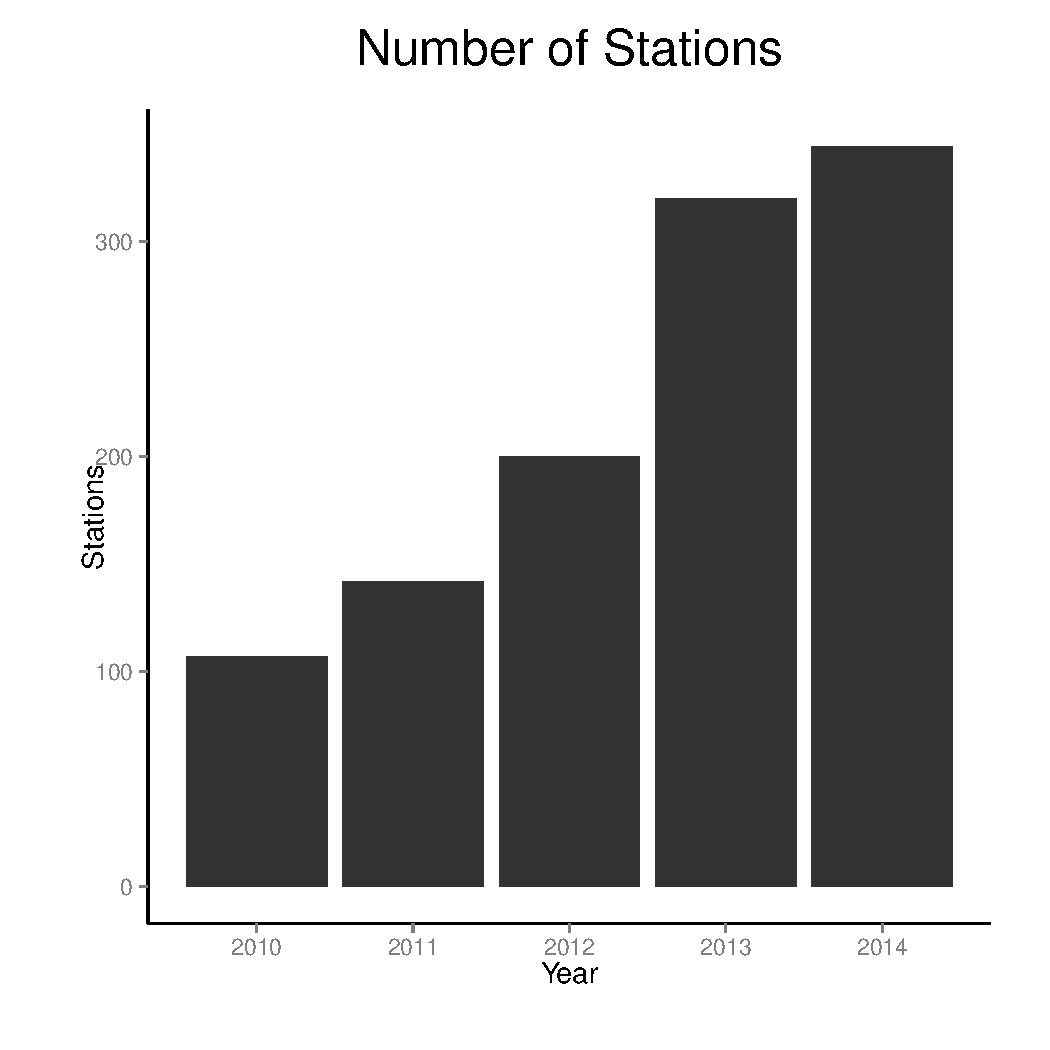
\includegraphics[scale=0.5]{../graphs/num_stations.pdf}
\end{minipage}

\begin{minipage}{.5\textwidth}
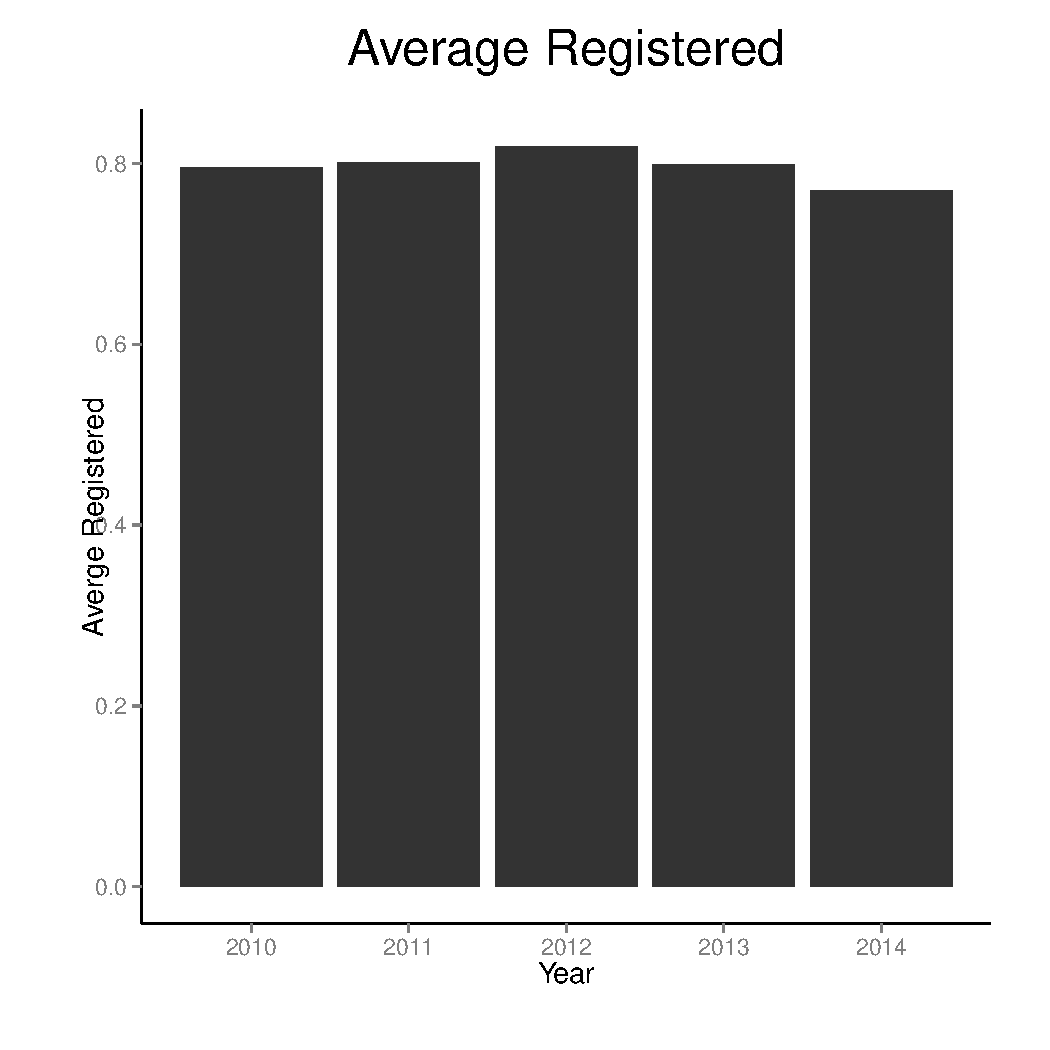
\includegraphics[scale=0.5]{../graphs/avg_reg.pdf}
\end{minipage}%
\begin{minipage}{.5\textwidth}
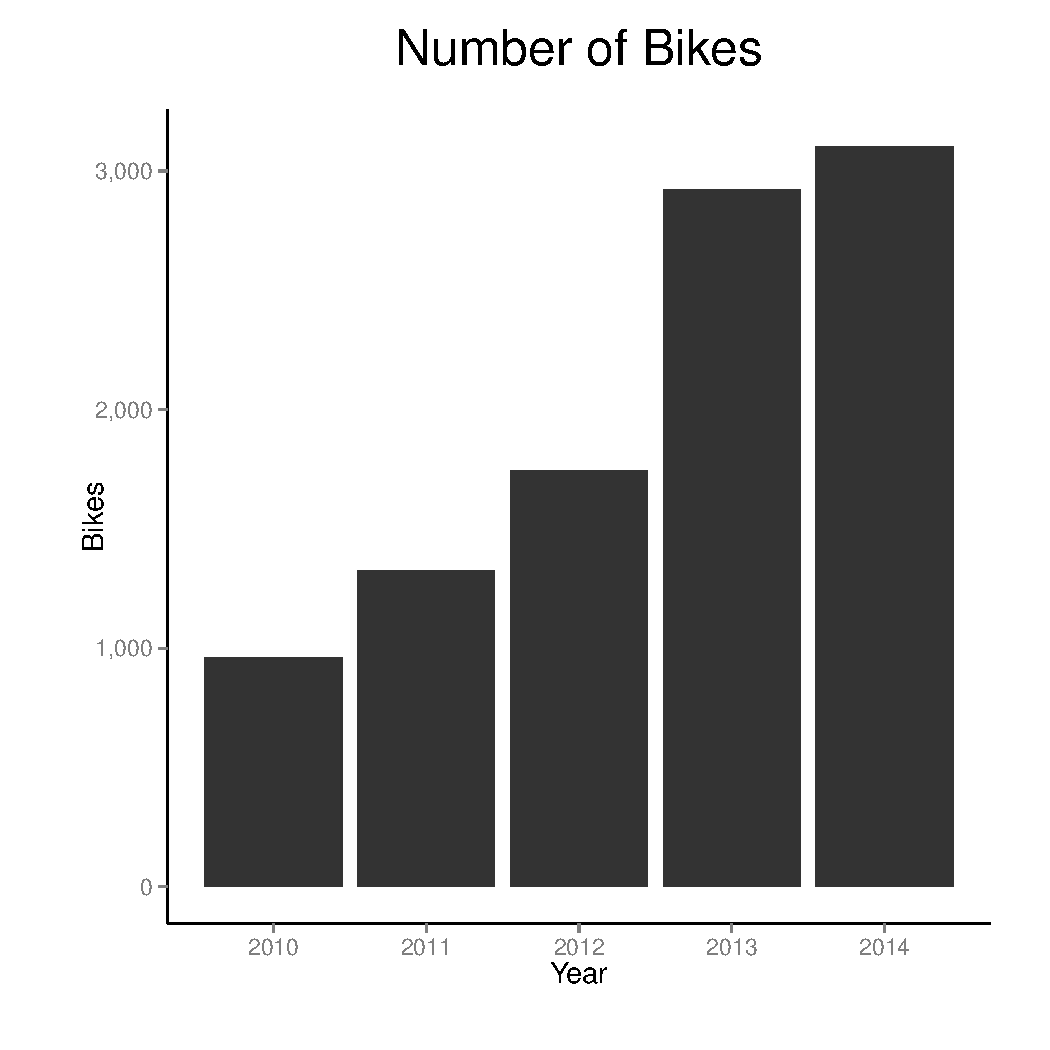
\includegraphics[scale=0.5]{../graphs/num_bikes.pdf}
\end{minipage}

\section{Membership Status Comparison}

\begin{minipage}{.5\textwidth}
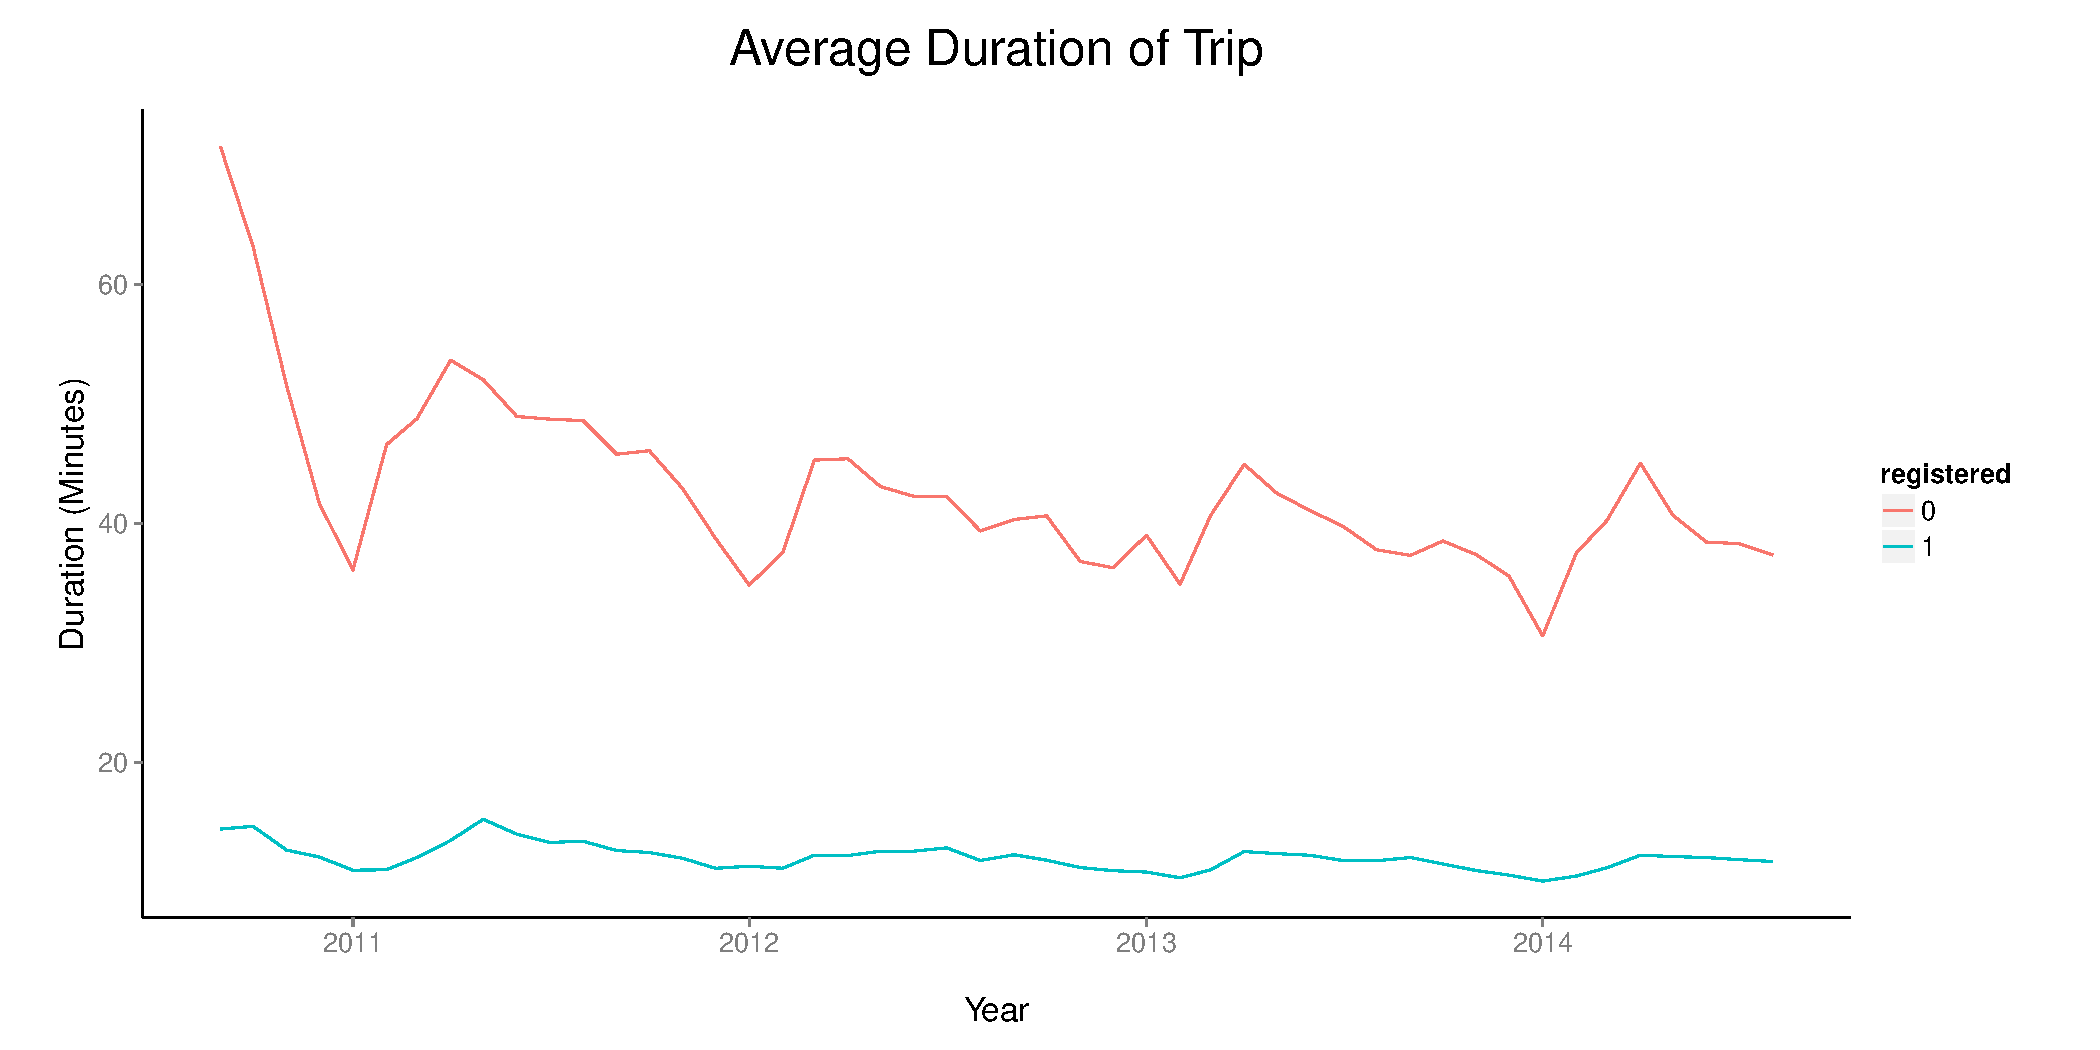
\includegraphics[scale=0.5]{../graphs/avg_duration_bytype.pdf}
\end{minipage}%
\begin{minipage}{.5\textwidth}

\includegraphics[scale=0.5]{../graphs/num_trips_bytype.pdf}
\end{minipage}

\section{OLS Regression Results}

 % Table created by stargazer v.5.1 by Marek Hlavac, Harvard University. E-mail: hlavac at fas.harvard.edu % Date and time: Tue, Feb 03, 2015 - 12:16:38 AM 
 \begin{table}[!htbp] 
\scriptsize 
 \centering    \caption{OLS Regression}    \label{}  \begin{tabular}{@{\extracolsep{5pt}}lc}  \\[-1.8ex]\hline  \hline \\[-1.8ex]   & \multicolumn{1}{c}{\textit{Dependent variable:}} \\  \cline{2-2}  \\[-1.8ex] & count \\  \hline \\[-1.8ex]   factor(season)2 & $-$2.465 \\    & (5.398) \\    & \\   factor(season)3 & $-$37.082$^{***}$ \\    & (6.902) \\    & \\   factor(season)4 & 65.159$^{***}$ \\    & (4.541) \\    & \\   holiday & $-$9.442 \\    & (9.177) \\    & \\   workingday & $-$2.705 \\    & (3.283) \\    & \\   factor(weather)2 & 14.020$^{***}$ \\    & (3.600) \\    & \\   factor(weather)3 & $-$9.167 \\    & (6.053) \\    & \\   factor(weather)4 & 185.765 \\    & (154.207) \\    & \\   temp & 8.096$^{***}$ \\    & (1.206) \\    & \\   atemp & 2.778$^{***}$ \\    & (1.058) \\    & \\   humidity & $-$2.810$^{***}$ \\    & (0.094) \\    & \\   windspeed & 0.596$^{***}$ \\    & (0.199) \\    & \\   Constant & 121.079$^{***}$ \\    & (9.042) \\    & \\  \hline \\[-1.8ex]  Observations & 10,886 \\  R$^{2}$ & 0.277 \\  Adjusted R$^{2}$ & 0.276 \\  Residual Std. Error & 154.137 (df = 10873) \\  F Statistic & 346.719$^{***}$ (df = 12; 10873) \\  \hline  \hline \\[-1.8ex]  \textit{Note:}  & \multicolumn{1}{r}{$^{*}$p$<$0.1; $^{**}$p$<$0.05; $^{***}$p$<$0.01} \\  \end{tabular}  \end{table} 

\end{document}